\section{Kernel Regression} 

  K nearest neighbor regression puts equal weights on both near and far points, as long as they are in the window. This may not be ideal, so a simple modification is to \textit{weigh} these points according to their distance from the middle $x$. We can do this with a kernel, as the name suggests. Now this is not the same thing as a Mercer kernel in RKHS, so to distinguish that I will call it a \textit{local averaging kernel}. 

  \begin{definition}[Local Averaging Kernel]
    A \textbf{kernel} is any smooth, symmetric, and non-negative function $K : \mathbb{R} \to \mathbb{R}$.  
  \end{definition}

  \begin{example}[Some Simple Kernels]
    Here are some popular kernels. 
    \begin{figure}[H]
      \centering
      \begin{subfigure}[b]{0.32\textwidth}
        \centering
        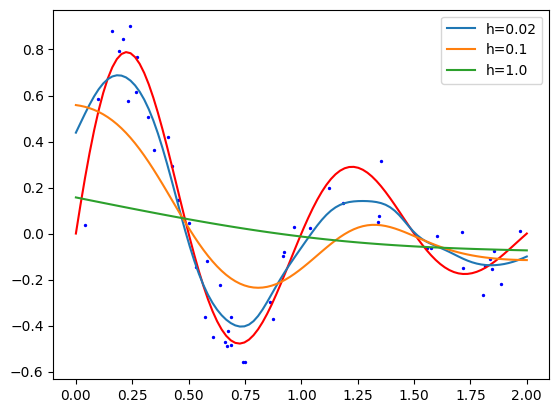
\includegraphics[scale=0.33]{img/gaussian_smoother.png}
        \caption{$K(x) = \frac{1}{\sqrt{2 \pi}} e^{-x^2/2}$. } 
        \label{fig:gaussian_smoother}
      \end{subfigure}
      \hfill 
      \begin{subfigure}[b]{0.32\textwidth}
        \centering
        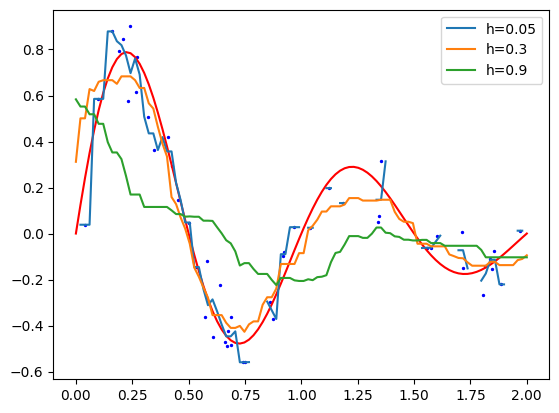
\includegraphics[scale=0.33]{img/boxcar_smoother.png}
        \caption{$K(x) = \frac{1}{2} \mathbbm{1}(|x| \leq 1)$.} 
        \label{fig:boxcar_smoother}
      \end{subfigure}
      \hfill 
      \begin{subfigure}[b]{0.32\textwidth}
        \centering
        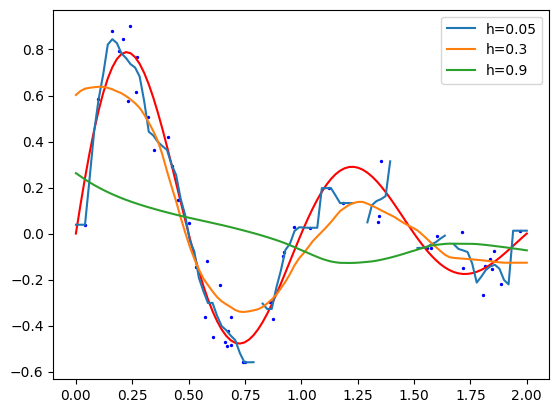
\includegraphics[scale=0.33]{img/epanechnikov_smoother.png}
        \caption{$K(x) = \frac{3}{4} (1 - x^2) \mathbbm{1}(|x| \leq 1)$.} 
        \label{fig:epanechnikov_smoother}
      \end{subfigure}
      \caption{The Gaussian, boxcar, and Epanechnikov kernels.}
    \end{figure}
  \end{example}
  
  The idea is to simply take the weighted average of the $y_i$'s. $\hat{f} (x) = \sum_{i} y_i \ell(x) \text{ where } \sum_{i} \ell_i (x) = 1$. The reason we'd like to have the weights to sum to $1$ is that if we had data that was constant (i.e. all $y_i$'s are the same), then the fitted function should be constant at that value as well. 

  \begin{definition}[Kernel Regression]
    Given a dataset $\mathcal{D} = \{(x^{(i)}, y^{(i)})\}_{i=1}^n$, a \textbf{kernel regression} model\footnote{Not to be confused with RKHS regression, or kernel ridge regression!}, or \textbf{local smoothing regression}, is a model of the form 
    \begin{equation}
      \hat{y} = f(x) = \frac{\sum_{i} y_i K \bigg( \frac{\|x - x_i\|}{h} \bigg)}{\sum_{i} K \bigg( \frac{\|x - x_i\|}{h} \bigg)}
    \end{equation}
    where $h$ is the \textbf{bandwidth} and the denominator is made sure so that the coefficients sum to $1$. Note that this function can have kernels defined at all points in $\mathcal{X}$, but it is interesting to examine it at the training points. 
  \end{definition}

  Denoting $y = (y_1, \ldots, y_n) \in \mathbb{R}^n$ and the vector $f(x) = (f(x_1), \ldots, f(x_n))$, if we can write the kernel function as $\hat{y} = \hat{f}(x) = S y$, which in matrix form, is 
  \begin{equation}
    \begin{bmatrix} \hat{y}_1 \\ \vdots \\ \hat{y}_n \end{bmatrix} = \begin{bmatrix} \hat{f}(x_1) \\ \vdots \\ \hat{f} (x_n) \end{bmatrix} = \begin{bmatrix} \ell_1 (x_1) & \cdots & \ell_n (x_1) \\ \vdots & \ddots & \vdots \\ \ell_1 (x_n) & \cdots & \ell_n (x_n) \end{bmatrix} \begin{bmatrix} y_1 \\ \vdots \\ y_n \end{bmatrix} 
  \end{equation}
  then we say that we have a \textbf{linear smoother}, with stochastic matrix $S$ being our \textbf{smoothing matrix}. 

  Furthermore, the theme of linearity is important and will be recurring. The kernel estimator is defined for all $x$, but it's important to see its behavior at the training points $x_i$. The estimator $\hat{y} = \hat{f}(x)$ is a linear combination of the $y_i$'s, and the coefficients $\ell_i (x_j)$ depend on the values of $x_j$. Therefore, we have $\hat{y} = S y$, which is very similar to the equation $\hat{y} = H y$ in linear regression, where $H$ is the hat matrix that projects $y$ onto the column space of $x$. Nonparametric regression has the same form, but rather than being a projection, it is a linear smoothing matrix. Therefore, this theme unifies both linear regression and nonparametric regression. Linear smoothers, spline smoother, Gaussian processes, are all just different choices of the smoothing matrix $S$. However, not all nonparametric estimators are linear smoothers, as we will see later. 

  \begin{example}[Gaussian Kernels in 1 Dimension]
    Let's perform Gaussian kernel regression on a dataset with 1 covariate and 1 response variable. It is quite robust. 
    
    \begin{lstlisting}
      import numpy as np
      import matplotlib.pyplot as plt

      def true_function(x):
        return 0.1 * x**4 - 0.5 * x**3 - x**2 + 2 * x + 1

      n_samples = 200
      X = np.random.uniform(-5, 5, n_samples)
      Y = true_function(X) + np.random.normal(0, 4.0, n_samples)

      def gaussian_kernel(u):
        return (1 / np.sqrt(2 * np.pi)) * np.exp(-0.5 * u**2)

      def kernel_regression(x, bandwidth):
        # Handle both scalar and array inputs
        x = np.atleast_1d(x)
        predictions = []
        
        for x_point in x:
          distances = (x_point - X) / bandwidth
          weights = gaussian_kernel(distances)
          prediction = np.sum(weights * Y) / np.sum(weights)
          predictions.append(prediction)
        
        return np.array(predictions)

      # Create evaluation points for smooth plotting
      x_space = np.linspace(-5, 5, 300)
      y_true = true_function(x_space)

      # Try different bandwidths
      bandwidths = [0.3, 0.8, 1.5]
      colors = ['red', 'green', 'blue']

      plt.figure(figsize=(12, 8))
      plt.scatter(X, Y, alpha=0.6, color='gray', s=20, label='Data points')
      plt.plot(x_space, y_true, 'black', linewidth=2, label='True function')

      for bandwidth, color in zip(bandwidths, colors):
        y_pred = kernel_regression(x_space, bandwidth)
        plt.plot(x_space, y_pred, color=color, linewidth=2, label=f'Gaussian Kernel (h={bandwidth})')

      plt.legend(fontsize=11)
      plt.grid(True, alpha=0.3)
      plt.xlim(-5, 5)
      plt.tight_layout()
      plt.show()
    \end{lstlisting}

    This produces the various estimates. 

    \begin{figure}[H]
      \centering 
      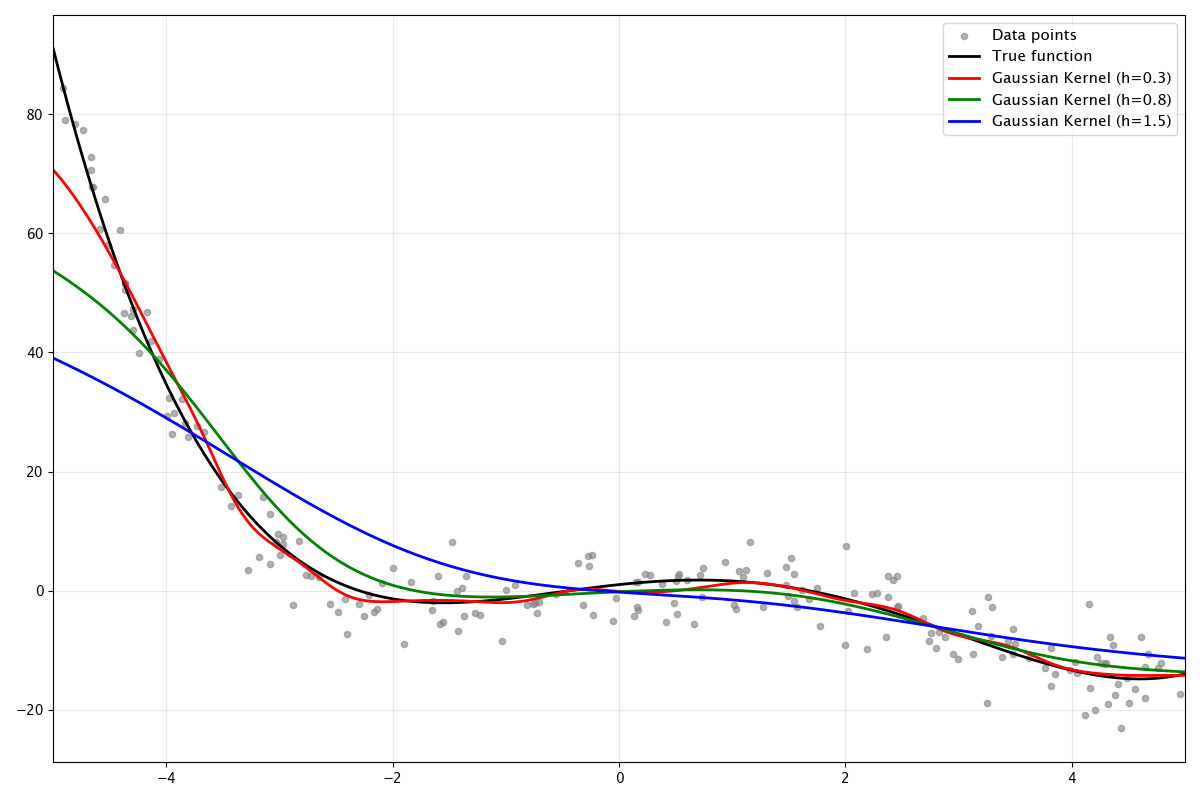
\includegraphics[scale=0.4]{img/kernel_reg_1d.png}
      \caption{Note that if $h$ is small (red), the line may be more sensitive to noise, leading to overfitting. } 
    \end{figure}
  \end{example}

  \begin{example}[Gaussian Kernels in 2 Dimensions] 
    Let's try to fit this for 2-dimensional covariates, with a much harder function now. 

    \begin{lstlisting}
      import numpy as np
      import matplotlib.pyplot as plt

      def true_function(x1, x2):
        return (2 * np.sin(x1) * np.cos(x2) + 
               1.5 * np.exp(-(x1**2 + x2**2)/8) + 
               0.8 * np.sin(2*x1) * np.sin(2*x2) +
               0.5 * np.cos(x1 + x2) - 
               0.3 * (x1**2 + x2**2)/10)

      n_samples = 300
      X1 = np.random.uniform(-5, 5, n_samples)
      X2 = np.random.uniform(-5, 5, n_samples)
      Y = true_function(X1, X2) + np.random.normal(0, 0.5, n_samples)

      def gaussian_kernel(u):
        return (1 / np.sqrt(2 * np.pi)) * np.exp(-0.5 * u**2)

      def kernel_regression_2d(x1, x2, bandwidth):
        x1 = np.atleast_1d(x1)
        x2 = np.atleast_1d(x2)
        predictions = []
        
        for x1_point, x2_point in zip(x1, x2):
          distances = np.sqrt((x1_point - X1)**2 + (x2_point - X2)**2) / bandwidth
          weights = gaussian_kernel(distances)
          prediction = np.sum(weights * Y) / np.sum(weights)
          predictions.append(prediction)
        
        return np.array(predictions)

      # Create evaluation grid
      x1_space = np.linspace(-5, 5, 40)
      x2_space = np.linspace(-5, 5, 40)
      X1_grid, X2_grid = np.meshgrid(x1_space, x2_space)
      x1_flat = X1_grid.flatten()
      x2_flat = X2_grid.flatten()

      # True function surface
      Y_true = true_function(X1_grid, X2_grid)

      # Figure 1: Data and True Function
      fig1 = plt.figure(figsize=(12, 5))

      ax1 = fig1.add_subplot(121, projection='3d')
      ax1.scatter(X1, X2, Y, alpha=0.6, s=15, c='gray')
      ax1.set_title('Training Data')
      ax1.set_xlabel('X1')
      ax1.set_ylabel('X2')
      ax1.set_zlabel('Y')

      ax2 = fig1.add_subplot(122, projection='3d')
      ax2.plot_surface(X1_grid, X2_grid, Y_true, alpha=0.9, cmap='viridis')
      ax2.set_title('True Function')
      ax2.set_xlabel('X1')
      ax2.set_ylabel('X2')
      ax2.set_zlabel('Y')

      plt.tight_layout()
      plt.show()

      # Figure 2: Kernel Regression with Different Bandwidths
      bandwidths = [0.3, 0.8, 1.5]
      fig2 = plt.figure(figsize=(15, 5))

      for i, bandwidth in enumerate(bandwidths):
       y_pred_flat = kernel_regression_2d(x1_flat, x2_flat, bandwidth)
       Y_pred = y_pred_flat.reshape(X1_grid.shape)
       
       ax = fig2.add_subplot(1, 3, i+1, projection='3d')
       ax.plot_surface(X1_grid, X2_grid, Y_pred, alpha=0.9, cmap='plasma')
       ax.set_title(f'Kernel Regression (h={bandwidth})')
       ax.set_xlabel('X1')
       ax.set_ylabel('X2')
       ax.set_zlabel('Y')

      plt.tight_layout()
      plt.show()
    \end{lstlisting}
    
    The dataset and the true function is shown. 

    \begin{figure}[H]
      \centering 
      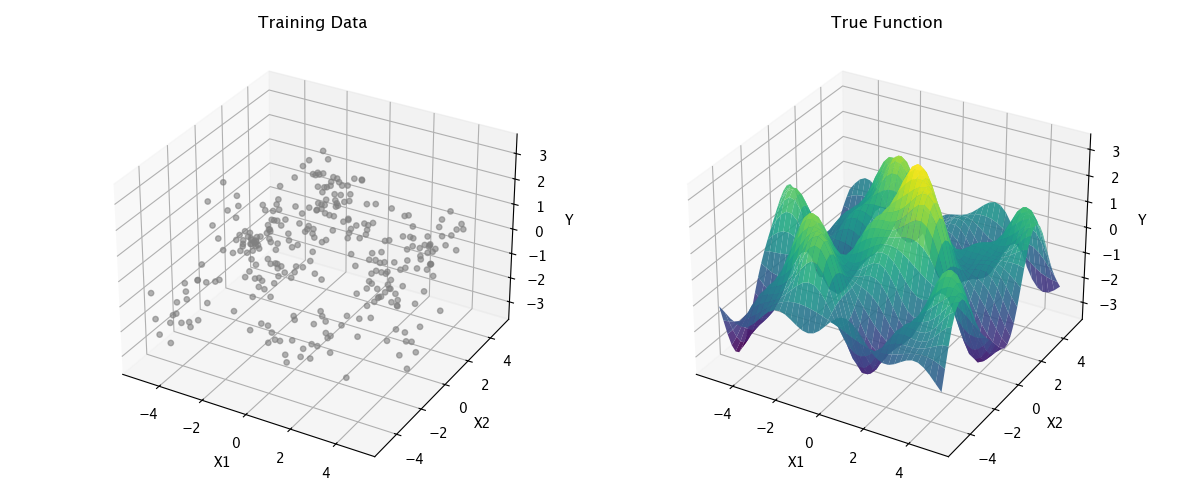
\includegraphics[scale=0.4]{img/kernel_reg_2d_true.png}
      \caption{} 
    \end{figure}

    Here are the fitted functions for many values. 

    \begin{figure}[H]
      \centering 
      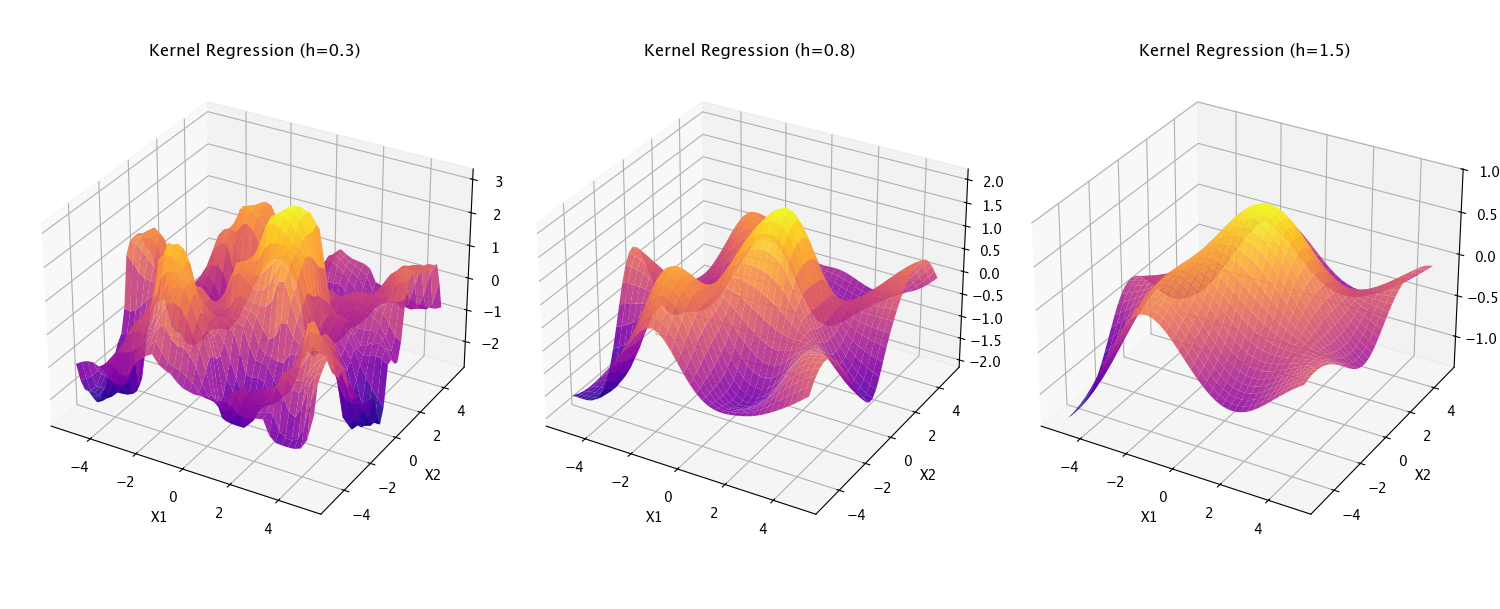
\includegraphics[scale=0.4]{img/kernel_reg_2d_est.png}
      \caption{} 
    \end{figure}
  \end{example} 

\subsection{Bias Variance Tradeoff}

  Just like we do with OLS, we want to minimize the MSE loss. It turns out that from a theoretical point of view, the choice of the kernel doesn't really matter. What really matters is the bandwidth $h$ since that is what determines the bias variance tradeoff. To see why, if $h = 0$, then it will simply interpolate the points and variance is extremely high, and if $h = \infty$, then the fitted function will be constant at $\bar{Y}$, leading to high bias. The following theorem formalizes this but for the simpler case of $d = 1$. 

  \begin{theorem}[Bias Variance Tradeoff of Kernel Regression]
    Suppose that $d = 1$ and that $m^{\prime\prime}$ is bounded. Also suppose that $X$ has a nonzero, differentiable density $p$ and that the support is unbounded. Then, the risk is 
    \begin{align}
      \mathbb{E}_{\mathcal{D}} \left[ (\hat{m}(x) - m(x))^2 \right] & = \frac{h^4}{4} \bigg( \int x^2 K(x) \bigg)^2 \int \bigg( m^{\prime\prime} (x) + 2m^\prime (x) \frac{p^\prime (x)}{p(x)} \bigg)^2 \,dx \\
          & \;\;\; + \frac{\sigma^2 \int K^2(x)\,dx} {n h_n} \int \frac{dx}{p(x)} + o \bigg( \frac{1}{n h_n} \bigg) + o(h_n^4) 
    \end{align}
    The first term is the squared bias and the second term is the variance. $p$ represents the density of $x$. 
  \end{theorem}
  \begin{proof}
    We first denote 
    \begin{equation}
      \hat{f}(X) = \frac{\frac{1}{nh} \sum_{i=1}^n K \bigg( \frac{X - X_i}{h} \bigg) Y_i}{\frac{1}{nh} \sum_{i=1}^n K \bigg( \frac{X - X_i}{h} \bigg)} 
    \end{equation}
    where the denominator is the kernel density estimator $\hat{p}(X)$. Therefore, we rewrite
    \begin{align}
      \hat{f} (x) - f(x) & = \frac{\hat{a}(x)}{\hat{p}(x)} - f(x) \\
                         & = \bigg( \frac{\hat{a}(x)}{\hat{p}(x)} - f(x) \bigg) \bigg( \frac{\hat{p}(x)}{p(x) + 1 - \frac{\hat{p}(x)}{p(x)}} \bigg) \\
                         & = \frac{\hat{a}(x) - f(x) \hat{p}(x)}{p(x)} + \frac{(\hat{f}(x) - f(x)) (p(x) - \hat{p}(x))}{p(x)}
    \end{align}
    as $n \rightarrow \infty$ both $\hat{f}(x) - f(x)$ and $p(x) - \hat{p}(x)$ going to $0$, and since they're multiplied in the second term, it will go to $0$ very fast. So the dominant term is the first term, and we can write the above as approximately 
    \begin{equation}
      \hat{f}(x) - f(x) \approx  \frac{\hat{a}(x) - f(x) \hat{p}(x)}{p(x)}
    \end{equation}
    TBD continued. Wasserman lecture 6, 10:00. 
  \end{proof}

  From the theorem above, we can see that if the bandwidth is small, then $h^4$ is small and the bias decreases. However, there is a $h$ term in the denominator of the variance term, which also trades it off. However, there are two problems. 
  \begin{enumerate}
    \item We can furthermore see that the bias is sensitive to $p^\prime / p(x)$. This means that if the density is steep, then the bias will be high. This is known as \textit{design bias}, which refers to bias stemming from how the $x$'s are distributed. 
    \item Another problem that is not contained in the theorem is the \textit{boundary bias}, which states that if you're near the boundary of the distribution (near the boundary of its support), then the bias also explodes. This happens to be very nasty especially in high dimensions where most of the data tends to be near the boundary.
  \end{enumerate}

  It turns out that this can be easily fixed with local polynomial regression, which gets rid of this term in the bias without any cost to variance. This means that this is unnecessary bias. 
